\documentclass[10pt,a4paper]{article}
\usepackage[utf8]{inputenc}
\usepackage[ngerman]{babel}
\selectlanguage{ngerman}
\usepackage{amsmath}
\usepackage{amsfonts}
\usepackage{amssymb}
\usepackage{graphicx}
\usepackage{booktabs}

\usepackage{algorithm}
\floatname{algorithm}{Algorithmus}
\usepackage[noend]{algpseudocode}
\usepackage{listings}
\lstset{language=C,stepnumber=1,numbers=left,breaklines=true}
\usepackage[shortcuts]{extdash}	% trenne auch Worte, die einen Bindestrich enthalten
\providecommand{\abs}[1]{\lvert#1\rvert}
\providecommand{\norm}[1]{\lVert#1\rVert}
\usepackage{graphicx}
\usepackage{hyperref}
\usepackage{color}
\newcommand{\algorithmautorefname}{Algorithmus}

\hyphenation{
RGBA
}

\begin{document}

\author{Christian Busch
\and
Igor Karlinskiy
\and
Oleksandr Khomenko
\and
Sascha Denis Knöpfle
}
\title{Portierung und Parallelisierung mehrerer Filter von GIMP nach GEGL}
\maketitle

\section{Einleitung}
Das Anwenden von Filtern auf Bilddaten ist ein häufiger Anwendungsfall für Parallelisierung. Hierbei muss oft ein und dieselbe Operation für jeden Pixel des Ausgabebildes angewandt werden. Somit lässt sich relativ einfach ein datenparalleler Algorithmus formulieren. Nachdem sich Mehrkernprozessoren sowohl in Desktop-PCs als auch in Laptops und sogar günstigen Netbooks und Smart Phones als Standard etabliert haben ist davon auszugehen, dass eine Mehrheit der Nutzer von GEGL mehrere Threads gleichzeitig ausführen kann.  Nicht zuletzt sind insbesondere Grafikkarten hervorragend für diese Aufgabe geeignet, wurden sie doch mit Hinblick auf jenes Szenario entwickelt. Im Zuge der fortschreitenden Marktdurchdringung von OpenCL ist davon auszugehen, dass ebenso die Anzahl der Nutzer, welche von einer Portierung der Algorithmen auf die GPU profitieren würden, wachsen wird. Es ergibt sich also ein hohes Potential durch Parallelisierung die Wartezeit der meisten Nutzer zu verringern.

Unsere Gruppe hat vier Filtern von GIMP nach GEGL portiert und parallelisiert. Für die Parallelisierung auf der CPU wurden OpenMP und SSE verwendet, ein Filter wurde zudem mittels OpenCL parallelisiert.
Die vorliegende Arbeit soll sowohl unsere Vorgehensweise und Erfahrung als auch die Ergebnisse der Portierung und Parallelisierung dokumentieren. 
%Standvorher
%Zielsetzung
%Portierung von GIMP nach GEGL
%Parallelisierung mittels OpenMP

\section{Filter}
\subsection{Color Exchange}
\paragraph{Filter aus Nutzersicht}
\glqq Dieses Filter ersetzt eine Farbe durch eine andere.\grqq\footnote{\url{http://docs.gimp.org/de/plug-in-exchange.html}} -- so steht es in der Dokumentation von GIMP und fasst die Grundidee des Filters grob zusammen. Tatsächlich ermöglicht das Filter jedoch nicht nur exakt eine Farbe durch eine andere zu ersetzen, sondern auch ähnliche Farben durch eine andere zu ersetzen. Somit können auch ganze Farbverläufe unter Beibehaltung der Abstufung mit einer anderen Farbe versehen werden.

\paragraph{Algorithmus} 

Das Filter prüft für jeden Pixel im Eingabebild jeweils für jeden Farbkanal ob der Farbwert nicht mehr als um den angegebenen Grenzwert von der Auswahlfarbe abweicht. Trifft dies zu wird jeweils der gewünschte Farbwert addiert mit dem positiven Betrag der Abweichung in das Ausgabebild geschrieben. Ist die Abweichung größer so wird der Wert dieses Farbkanals für jenen Pixel unverändert in das Ausgabebild übertragen. Ebenfalls unverändert bleibt der Alpha-Wert eines jeden Pixels.

\begin{algorithm}[H]
\caption{Pseudo-Code des \glqq Color Exchange\grqq-Algorithmus}
\label{algo:exchange}
\begin{algorithmic}[1]
\State $color \in \{red, green, blue\}$
\ForAll{$pixel \in input$}
  \State $\delta_{color} \gets \abs{ pixel_{color} - from_{color}}$    
  \If{$\forall color: \delta_{color} \leq threshold_{color}$}
    \ForAll{$color$}  
      \State $outputPixel_{color} \gets from_{color} + \delta_{color}$
    \EndFor
  \Else
    \ForAll{$color$}
      \State $outputPixel_{color} \gets pixel_{color}$
    \EndFor
  \EndIf
  \State $outputPixel_{alpha} \gets pixel_{alpha}$
  \State schreibe $outputPixel$ in das Ausgabebild
\EndFor
\end{algorithmic}
\end{algorithm}

\paragraph{Portierung}
Bei der Portierung wurde vorerst die Farbrepräsentation in R'G'B'A mit 8 Bit je Farbkanal beibehalten. Ferner enthält die Implementierung innerhalb von GIMP bereits einen Fehler. Dieser wurde bei der Portierung ebenfalls übernommen um einen Vergleich zwischen portierter und der ursprünglichen Variante dieses Filters ziehen zu können. Die fragliche Code-Stelle findet sich in Zeile 6 von \autoref{algo:exchange}. Durch die Verwendung des Betrages der Differenz an jener Stelle führen insbesondere hohe Schwellwerte zu unerwünschten Artefakten. Der Fehler wurde bereits den GEGL-Entwicklern mitgeteilt und wird von uns zu einem späteren Zeitpunkt korrigiert.

\paragraph{Parallelisierung}
Bei diesem Filter handelt es sich um einen sogenannten Punktfilter, was bedeutet, dass ein Ausgabepixel von genau einem Eingabepixel abhängt. Somit ist keine Koordination zwischen den einzelnen Threads notwendig. Dies ist ein glücklicher Umstand für die Parallalisierung, da diese besonders einfach ausfällt. So einfach, dass diese Klasse von Problemen in der Fachsprache \glqq embarassingly parallel\grqq also etwa \glqq peinlich parallel\grqq genannt wird.

Zur Parallelisierung wurde OpenMP verwendet. Hierbei wurde das Eingabebild in (nicht zwangsläufig zusammenhängenden) Streifen auf die jeweiligen Threads aufgeteilt. Ein Thread berechnet somit jeweils einen oder mehrere Streifen aus beieinander liegenden Pixeln.

\begin{algorithm}[H]
\caption{Pseudo-Code des \glqq Color Exchange\grqq-Algorithmus in OpenMP}
\label{algo:exchange_par}
\begin{algorithmic}[1]
\State $color \in \{red, green, blue\}$
\State zerlege Bild in numThreads Teilbereiche
\State weise jedem Thread seinen Teilbereich $threadInput$ zu
\ForAll{$thread \in {1..numThreads}$}
\ForAll{$pixel \in threadInput_{thread}$}
  \State $\delta_{color} \gets \abs{ pixel_{color} - from_{color}}$    
  \If{$\forall color: \delta_{color} \leq threshold_{color}$}
    \ForAll{$color$}  
      \State $outputPixel_{color} \gets from_{color} + \delta_{color}$
    \EndFor
  \Else
    \ForAll{$color$}
      \State $outputPixel_{color} \gets pixel_{color}$
    \EndFor
  \EndIf
  \State $outputPixel_{alpha} \gets pixel_{alpha}$
  \State schreibe $outputPixel$ in das Ausgabebild
\EndFor
\EndFor
\end{algorithmic}
\end{algorithm}
 
Eine weitere Möglichkeit zur Parallelisierung bestünde darin jeweils die Betrachtung der Farbkanäle eines Pixels zu Parallelisieren. Diese Idee wurde jedoch als zu kleinschrittig verworfen. Der Koordinierungsaufwand (Threads starten, stoppen, etc.) für die Threads dürfte den Zeitgewinn bei der Berechnung mehr als aufwiegen. Denkbar wäre es jedoch diese Parallelisierung mittels Vektoreinheiten der CPU durchzuführen, also beispielsweise SSE zu verwenden.

Weiterhin gestaltet sich eine Parallelisierung mittels OpenCL recht einfach. Hierfür wählt man eine eindimmensionale Organisierung der Work Items und bearbeitet pro Work Item genau einen Pixel. Die äußere Schleife des sequenziellen Algorithmus fällt somit weg. Die oberen und unteren Grenzwerte werden einmal auf der CPU berechnet und der GPU als Konstanten übergeben. Diese Implementierung wäre sehr wahrscheinlich durch die Speicherbandbreite auf der GPU und durch die Bandbreite zwischen Host und GPU limitiert, da sehr wenige Berechnungen auf den Daten ausgeführt werden.



%% gtile_part.tex
\newpage
\subsection{Glass Tile}

\paragraph{Beschreibung des Filters aus Nutzersicht}

Dieses Filter lässt das Bild erscheinen, als würde es durch eine Wand aus Glasbausteinen betrachtet werden. Das Filter kann auf die aktive Ebene oder eine im Bild befindliche Auswahl angewendet werden.\footnote{\url{http://docs.gimp.org/de/plug-in-glasstile.html}} Die Kachelbreite und Kachelhöhe sind individuell einstellbar.

\paragraph{Algorithmus}

%Pseudocode, visuell
\begin{algorithm}[h]
\caption{Pseudo-Code des \glqq Glass Tile\grqq-Algorithmus}
\label{algo:gtile}
\begin{algorithmic}[1]
\State $xhalf \gets tileWidth  / 2$
\State $yhalf \gets tileHeight / 2$
\State $xplus \gets tileWidth  \mod 2$
\State $yplus \gets tileHeight \mod 2$
\State $ymiddle \gets 0$
\State $yoffs \gets 0$
\ForAll{$rows$ $r$ $\in input$}
	\State $ypixel2 \gets ymiddle + yoffs * 2$
	\State lese Zeile $ypixel2$ aus dem Eingabebild
	\State $yoffs$++
	\If{$yoffs = yhalf$}
		\State{$ymiddle \gets ymiddle + tileHeight$}
		\State{$yoffs \gets - (yhalf + yplus)$}
	\EndIf
	\State $xmiddle \gets 0$
	\State $xoffs \gets 0$
	\ForAll{$columns \in column$}
		\State $xpixel1 \gets (xmiddle + xoffs)$
		\State $xpixel2 \gets (xmiddle + xoffs * 2)$
		\State schreibe Pixel $xpixel2$ aus Eingabezeile nach $xpixel1$ in Ausgabezeile
		\State $xoffs$++
		\If{$xoffs = xhalf$}
			\State{$xmiddle \gets xmiddle + tileWidth$}
			\State{$xoffs \gets - (xhalf + xplus)$}
		\EndIf
	\EndFor
	\State speichere Ausgabezeile an Zeilenposition $r$ im Ausgabebild
\EndFor	
\end{algorithmic}
\end{algorithm}

%Beschreibung Algorithmus allgemeinsprachlich
\begin{figure}[h]
\begin{center}
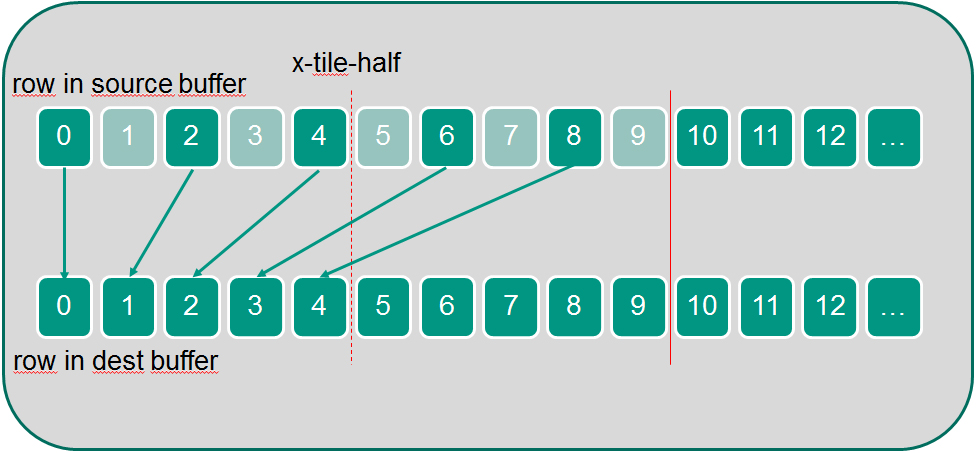
\includegraphics[width=0.95\textwidth]{gtile1.png}
\end{center}
\caption{Verrückung der Spalten innerhalb einer Zeile}\label{fig:gtile1}
\end{figure}
Der Algorithmus erzeugt sowohl zeilenweise als auch spaltenweise eine Verrückung und Wiederholung innerhalb der Kacheln. Dabei wird jede zweite Zeile in einer Kachel hintereinander in die erste Hälfte der Kachel verschoben wie in Abbildung~\ref{fig:gtile1} zu sehen.\newline
\begin{figure}[h]
\begin{center}
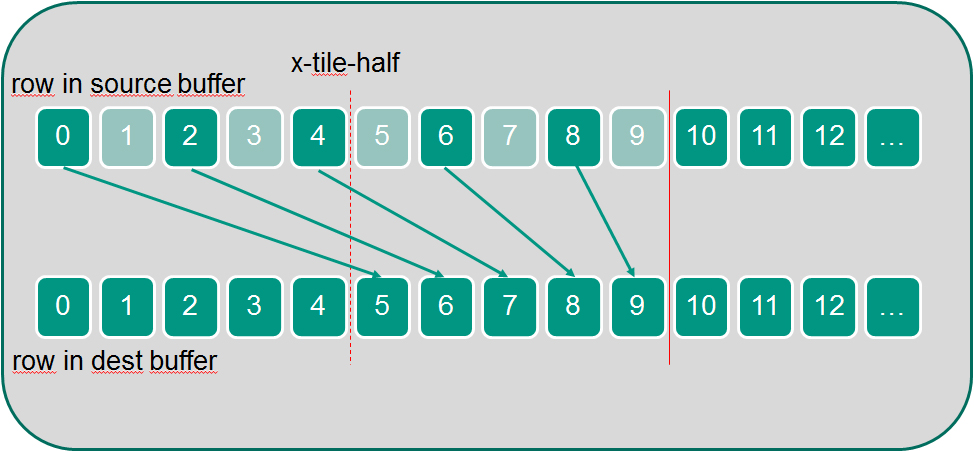
\includegraphics[width=0.95\textwidth]{gtile2.png}
\end{center}
\caption{Wiederholung der verrückten Spalten innerhalb einer Kachelzeile}\label{fig:gtile2}
\end{figure}
Diese gelesenen und verschobenen Zeilen werden anschließend in der zweiten Hälfte nochmals wiederholt, was in Abbildung~\ref{fig:gtile2} dargestellt ist.\newline
Die Verrückung und Wiederholung der Spalten erfolgt analog. Auf diese Weise wird Kachel für Kachel bearbeitet. Der sequentielle original Algorithmus liest dabei komplette Zeilen ein und führt darauf die notwendigen Spaltenverschiebungen durch.

\paragraph{Portierung}
Bei der Portierung wurde etwas getan.

\paragraph{Parallelisierung}
Peinlich peinlich möchte man denken.



%% edge-neon.tex
\newpage
\subsection{Neon}
\label{paragraph:neon_filter}
\paragraph{Filter aus Nutzersicht}
Dieses Filter extrahiert Kanten in der aktiven Ebene oder Auswahl und 
umgibt diese mit einem neonartigen Glühen.








\paragraph{Algorithmus} 
%Beschreibung Algorithmus allgemeinsprachlich, 
%Pseudocode, visuell
\begin{algorithm}[h]
\caption{Pseudo-Code des \glqq Neon\grqq-Algorithmus}
\label{algo:neon}
\begin{algorithmic}[1]
\ForAll{$columns \in input$}
	\State lese eine Spalte aus dem Eingabebild
	\ForAll{$pixel \in column$}
		\State berechne neon von oben nach unten
	\EndFor
	\ForAll{$pixel \in column$}
		\State berechne neon von unten nach oben
	\EndFor
	\State merge Ergebnisse in eine Spalte
	\State speichere in Ausgabebild
\EndFor	
\ForAll{$rows \in input$}
	\State lese eine Zeile aus dem Eingabebild
	\ForAll{$pixel \in row$}
		\State berechne neon von links nach rechts
	\EndFor
	\ForAll{$pixel \in row$}
		\State berechne neon von rechts nach links
	\EndFor	
	\State merge Ergebnisse in eine Zeile
	\State \label{neon_datenabhaengigkeit} bilde Gradient von dieser Zeile und einer aus dem Ausgabebild
	\State speichere in Ausgabebild
\EndFor
\end{algorithmic}
\end{algorithm}

Der Algorithmus besteht aus 2 großen Schleifen (detaillierterer Pseudo-Code 
ist in Algorithmus \ref{algo:neon} zu finden).
Beide Suchstufen (in jeder Schleife) erfolgen spalten- bzw. zeilenweise, und zwar von beiden Seiten simultan,
so ist in diesem Fall recht unbeliebte automatische Kachelzerlegung sehr vorteilhaft, da sie Wahrscheinlichkeit dafür erhöht, dass die zum Mergen benötigten Werte noch in Cache zu finden sind.

Für weitere Details siehe Paragraph ``Parallelisierung''.


















\paragraph{Portierung}
\label{neon_portierung}
Der ursprüngliche Code konnte zum größten Teil übernommen werden, natürlich nicht ohne Anpassung der Standardkonstrukte und Schnittstellen.
Auch mehrere unnötige bzw. überflüssige Sprachkonstrukte konnten erkannt und entfernt werden: z.B. mehrfache Abfrage ob Radius unter 1.

Des Weiteren wurden im Code viele Variablen umbenannt, was der Qualität und vor allem der Lesbarkeit beitrug, da bevor viele von denen wenigen buchstaben bestanden bzw. aus einer unbekannter Sprache stammen (\emph{sp\_p} in \emph{head\_buf}).

Beachten Sie bitte Hinweise in Paragraf Korrektheit\ref{paragraph:neon_korrektheit}.
















\paragraph{Parallelisierung}
Es gab auch ursprünglich keine funktionale Abhängigkeit zwischen den beiden Stufen (beide äußere For-Schleifen),  jedoch ließ sich der Algorithmus trotzdem nur bedingt parallelisieren. Grund dafür war eine Datenabhängigkeit: In der \ref{neon_datenabhaengigkeit}. Zeile des Algorithmus \ref{algo:neon} werden Ergebnisse der beiden Schritte zusammengeführt. Im sequenziellen Fall hätte es einen guten Grund - bessere Cacheausnutzung - ein der beiden benötigten Felder ist garantiert im Cache (so weit Cache ausreicht) vorhanden.

Wird der Algorithmus parallel ausgeführt, so sollte diese Datenabhängigkeit z.B. durch temporäre Variablen eliminiert werden. 


\subparagraph{Ansätze zur Parallelisierung}
\begin{enumerate}
	\item [] \begin{description} %Platzhalter links
		\item[1) Sections] Der ursprünglich verfolgte Ansatz. Beide äußere Schleifen werden durch ``\#pragma omp sections'' simultan abgearbeitet. Des Weiteren kann auch jede der Schleifen intern parallelisiert werden. Datenabhängigkeit muss eliminiert werden. Siehe Algorithmus \ref{algo:neon_sections}.
		
		Vorteile:
		\begin{itemize}
		\item[\texttt{+}] weniger Datenabhängigkeiten
		\item[\texttt{+}] kritischer Abschnitt ist außerhalb der parallelen Region
		\end{itemize}
		
		Nachteile:
		\begin{itemize}
		\item[\texttt{-}] schlechtere Cache-Ausnutzung
		\item[\texttt{-}] höherer Speicherbedarf (zusätzlicher GeglBuffer nötig)
		\end{itemize}
		

		\item[2) Konservative Schleifenparallelisierung] Unter Annahme, dass die vorhandene Datenabhängigkeit zwecks der besseren Cache-Ausnutzung beibehalten werden soll, muss die erste For-Schleife vollständig abgearbeitet sein, bevor es mit der Zweiten angefangen werden kann (implizite Barriere kann hier gute Dienste leisten). Siehe Algorithmus \ref{algo:neon_conservative}

		Vorteile:
		\begin{itemize}
		\item[\texttt{+}] bessere Cache-Ausnutzung
		\item[\texttt{+}] weniger Eingriffe in den Code
		\end{itemize}
		
		Nachteile:
		\begin{itemize}
		\item[\texttt{-}] kritischer Abschnitt innerhalb der parallelen Region 
		\end{itemize}
	\end{description}
\end{enumerate}

Da GEGL-eigene Methoden zum Lesen und vor allem Schreiben in Ausgabebild als not-thread-safe betrachtet werden und stark gewünscht sind, müssen sie in einem kritischen Bereich geschützt werden.
Der einzige Kritikpunkt an Algorithmus \ref{algo:neon_conservative} besteht darin, dass der kritische Bereich sich in der parallelen Region befindet, was hier zum Flaschenhals resultieren wird - mit zunehmender Threadzahl wird die Effizienz schnell fallen.

Beide Ansätze sind mithilfe von OpenMP realisiert.





\newpage
%PARALLELISIERUNG MIT SECTIONS
\begin{algorithm}[H]
\caption{Pseudo-Code des \glqq Neon\grqq-Algorithmus: Sections}
\label{algo:neon_sections}
\begin{algorithmic}[1]
\State \textcolor{blue}{\#pragma omp parallel sections}\{
\State \textcolor{blue}{\#pragma omp section} 
\ForAll{$columns \in input$}
	\State lese eine Spalte aus dem Eingabebild
	\ForAll{$pixel \in column$}
		\State berechne neon von oben nach unten
	\EndFor
	\ForAll{$pixel \in column$}
		\State berechne neon von unten nach oben
	\EndFor
	\State merge Ergebnisse in eine Spalte
	\State speichere in \textcolor{blue}{temporäres Feld1}
\EndFor	
\State \textcolor{blue}{\#pragma omp section}
\ForAll{$rows \in input$}
	\State lese eine Zeile aus dem Eingabebild
	\ForAll{$pixel \in row$}
		\State berechne neon von links nach rechts
	\EndFor
	\ForAll{$pixel \in row$}
		\State berechne neon von rechts nach links
	\EndFor	
	
		\State merge Ergebnisse in eine Zeile
	\State speichere in \textcolor{blue}{temporäres Feld2}
\EndFor
\State \}
\State \textcolor{blue}{\#pragma omp parallel for }
\ForAll{$pixel \in Ausgabebild$}
	\State \label{neon_keine_datenabhaengigkeit} lese je ein Pixel aus Feld1 und Feld2,  speichere Gradient in Ausgabebild
\EndFor
\end{algorithmic}
\end{algorithm}

%KONSERVATIVE PARALLELISIERUNG
\begin{algorithm}[H]
\caption{Pseudo-Code des \glqq Neon\grqq-Algorithmus: Konservative Schleifenparallelisierung}
\label{algo:neon_conservative}
\begin{algorithmic}[1]
\State \textcolor{blue}{\#pragma omp parallel for }
\ForAll{$columns \in input$}
	\State lese eine Spalte aus dem Eingabebild
	\ForAll{$pixel \in column$}
		\State berechne neon von oben nach unten
	\EndFor
	\ForAll{$pixel \in column$}
		\State berechne neon von unten nach oben
	\EndFor
	\State merge Ergebnisse in eine Spalte
	\State speichere in Ausgabebild
\EndFor	


\State \textcolor{blue}{\#pragma omp parallel for }
\ForAll{$rows \in input$}
	\State lese eine Zeile aus dem Eingabebild
	\ForAll{$pixel \in row$}
		\State berechne neon von links nach rechts
	\EndFor
	\ForAll{$pixel \in row$}
		\State berechne neon von rechts nach links
	\EndFor	
		\State merge Ergebnisse in eine Zeile
	\State bilde Gradient von dieser Zeile und einer aus dem Ausgabebild
	\State speichere in Ausgabebild
\EndFor
\end{algorithmic}
\end{algorithm}








%\begin{figure}
%\centering
%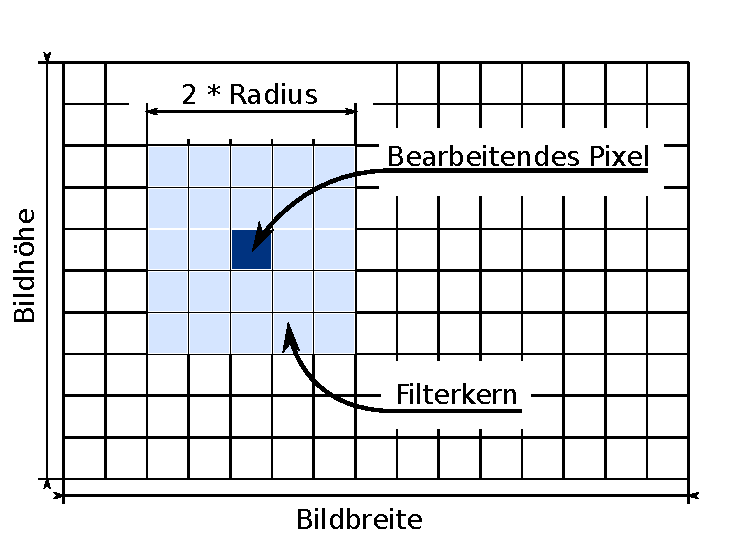
\includegraphics[scale=0.9]{graphs/sgb-grid.pdf}
%\caption{Selective Gaussian Blur. Schematische Darstellung}
%\label{fig:sgb-grid}
%\end{figure} 






















\subsection{Selective Gaussian Blur}
\paragraph{Filter aus Nutzersicht}
\paragraph{Algorithmus} 
%Beschreibung Algorithmus allgemeinsprachlich, 
%Pseudocode, visuell
\paragraph{Portierung}
\paragraph{Parallelisierung}
\subparagraph{OpenMP}
\subparagraph{OpenCL}
Dieses Filter wurde im Gegensatz zu den anderen Filtern nicht nur mittels OpenMP sondern auch mittels OpenCL parallelisiert. 


Durch die Portierung des Algorithmus nach OpenCL fielen die äußeren beiden Schleifen weg, da die Iteration über alle Pixel durch die Abbildung auf die Work Items erfolgte. Die Work Items wurden zweidimensional indiziert und es ist genau ein Work Item für genau einen Pixel zuständig.
Es wurden wo möglich Vector-Datentypen (float4) verwendet um sowohl Speicherzugriffe zu optimieren als auch um von der Nutzung der Vector-Recheneinheiten zu profitieren.

Durch die Zuordnung eines Pixels zu genau einem Work Item, wobei der Index beider identisch ist, ergibt sich ferner ein Zugriff auf den Globalen Speicher, der Speichertransfers optimiert. Benachbarte Work Items greifen auf benachbarte Speicherstellen zu. Somit kann der Speicherzugriff verschmolzen (coalesced) stattfinden was dazu führt, dass statt mehrerer kleiner Speicherzugriffe deutlich weniger größere erfolgen. Als Folge dessen wird die Speicherbandbreite besser genutzt, wodurch sich wiederum die Laufzeit verringert.

Nach der Implementierung mit jenen Optimierungen wurde die Laufzeit gemessen. Als sich herausstellte dass weitere Optimierungen kaum noch eine Verringerung der Laufzeit herbeiführen würden, da der Kernel bereits zu diesem Zeitpunkt nur noch einen kleinen Bruchteil der Gesamtlaufzeit der GEGL-Operation ausmachte (siehe Ahmdal's Law) wurde von weiteren Optimierungen abgesehen.

Weitere Ansätze zur Optimierung wären gewesen:
\begin{enumerate}
%% \item [] \begin{description} 
\item Durch die Verwendung lokalen Speichers ist es möglich die Speicherzugriffe auf den globalen Speicher zu minimieren. Da letzterer eine um Größenordnungen höhere Latenz hat als lokaler Speicher hätte man so bereits selbst bei nur einer Wiederverwendung der Daten eine insgesamt geringere Laufzeit. Hierbei ist jedoch zu beachten, dass lokaler Speicher nur in einer sehr begrenzten Größe zur Verfügung steht und jeweils nur von der Work Group verwendet werden kann, zu der er gehört. Daraus ergeben sich mehrere Konsequenzen:

Das Bild wird in mehrere Teilbilder zerlegt, deren Anzahl gleich der Zahl der Work Groups ist. Dies stellt zunächst einmal kein Problem dar. Jedoch benötigt dieses Filter für die Berechnung eines Pixels auch Pixel in seiner Umgebung. Mit zunehmender Größe dieser Umgebung, also zunehmendem Radius des Filters, erhöht sich ebenso die Redundanz der vorgehaltenen Pixel.



% Bild einfügen

Dies führt zu mehr Zugriffen auf den globalen Speicher, was somit die eigensparte Laufzeit wieder ein Stück weit aufzehrt, wenn dies nicht durch Latency Hiding also das "Verschleiern" der Latenz durch die Überbrückung der Wartezeit für Speicherzugriffe durch andere Operationen vermieden werden kann.
Darüber hinaus wächst aber auch der Speicherverbrauch an lokalem Speicher. Bei großen Radien führt dies dazu, dass weniger Work Units gleichzeitig ausgeführt werden können. Dies wiederum hat einen negativen Einfluss auf das Latency Hiding, da weniger Arbeit für das Überbrücken der Wartezeiten durch Speicherzugriffe vorhanden ist. 


% Bild einfügen?

Große Radien können weiterhin dazu führen, dass die zur Berechnung notwendige Umgebung (Halo) nicht vollständig in den lokalen Speicher passt. Somit wird ein aufwändigeres Speichermanagement notwendig. Die Größe des Radius ab dem diese Problematik auftritt lässt sich jedoch mit einer weiteren Optimierung zumindest erhöhen.


\item Eine weitere angedachte Optimierung war die Zerlegung des Filters in zwei Filter, die nacheinander aufgerufen werden. Man kann diesen Filter in eine horizontale und eine vertikale Operation zerlegen. Somit benötigt man nur noch die Umgebung in einer Ausrichtung (horizontal oder vertikal) in dem jeweiligen Filter. Dies spart Speicherzugriffe. Erschwerend kommt bei diesem Filter jedoch hinzu, dass man von einem Filter zum nächsten auch die Koeffizienten pro Pixel ebenfalls mitführen müsste -- entweder über einen seperaten Buffer oder aber gemeinsam in einem Buffer zusammen mit den Farbwerten. Ersteres ist hierbei in Hinblick auf das Speicher-Alignment vermutlich vorzuziehen, dies müsste man jedoch empirisch überprüfen.

% Bild einfügen.	Vorteil: Höhere Geschwindigkeit

\item Kombiniert man nun die Zerlegung des Filters in eine horizontalen und einen vertikalen mit der Nutzung lokalen Speichers, so ergeben sich Synergieeffekte. Es können nun die Halos größerer Radien im lokalen Speicher Platz finden.

\item Ist der Radius des Filters klein, so kann man nun zusätzlich zu den genannten Optimierungen auch noch mehrere Pixel pro Work Unit berechnen. Dies hat den Vorteil, dass sich das Verhältnis von berechneten Pixeln zu Halo-Pixeln zugunsten ersteren verschiebt. Somit verringert sich die Redundanz der im lokalen Speicher vorgehaltenen Pixel weiter und es werden weniger Daten vom globalen Speicher gelesen. Man müsste bei dieser Optimierung allerdings überprüfen wie viel lokalen Speicher man verwenden kann bevor die Laufzeit eventuell wieder steigt, da nicht mehr genug Work Items für Latency Hiding zur Verfügung stehen.
%%\end{description}
\end{enumerate}

\section{Evaluation der Ergebnisse}
\subsection{Color Exchange}
\paragraph{Korrektheit}
Der GEGL-Filter führt innerhalb GIMP bei gleichen Parametern zu den selben Ergebnissen wie der ursprüngliche GIMP-Filter. Der Aufruf über Konsole / XML-Datei gestaltet sich jedoch schwierig, da die Parameter-Übergabe augenscheinlich im falschen Farbraum stattfindet. Es scheint, als würden die per XML-Datei übergebenen Farbwerte im Format RGBA übergeben, aber als R'G'B'A interpretiert. Dies führt dazu, dass übergebene Farben sehr deutlich verfälscht werden. Eine elegante Möglichkeit zur Umgehung dieses Problems ist uns bisher nicht bekannt. Möglich wäre zwar einen weiteren Parameter (Farbraum) einzuführen, doch dies würde dazu führen, dass auch in der GUI ein weiterer, dort nicht benötigter, Parameter hinzu kommt. Es ist natürlich möglich zwischen den Farbräumen zu konvertieren, doch wäre es weder intuitiv noch bequem für den Nutzer. Somit sollte man den Filter aktuell als nur für die Verwendung innerhalb von GIMP gedacht verstehen.
\begin{figure}[H]
\centering
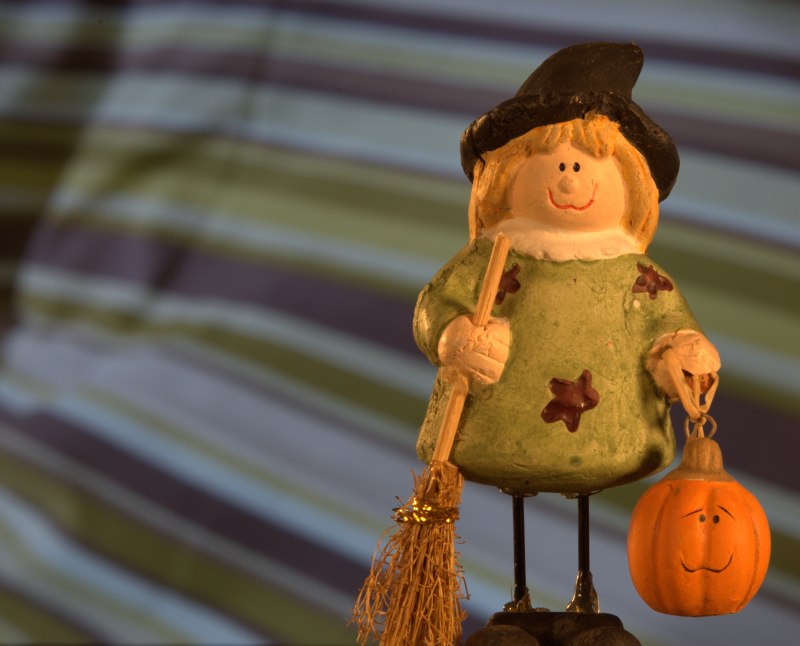
\includegraphics[scale=0.4]{img/matting-global.png}
\caption{Ausgangsbild}
\label{fig:CE_aus}
\end{figure}
\begin{figure}[H]
\centering
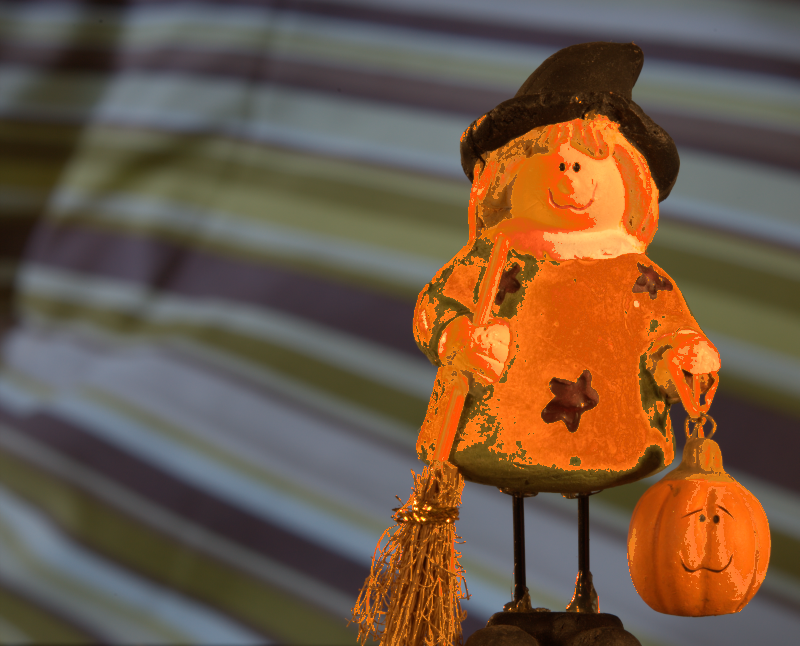
\includegraphics[scale=0.4]{img/matting-global_gimp.png}
\caption{Resultat der GIMP-Operation}
\label{fig:CE_gimp}
\end{figure}
\begin{figure}[H]
\centering
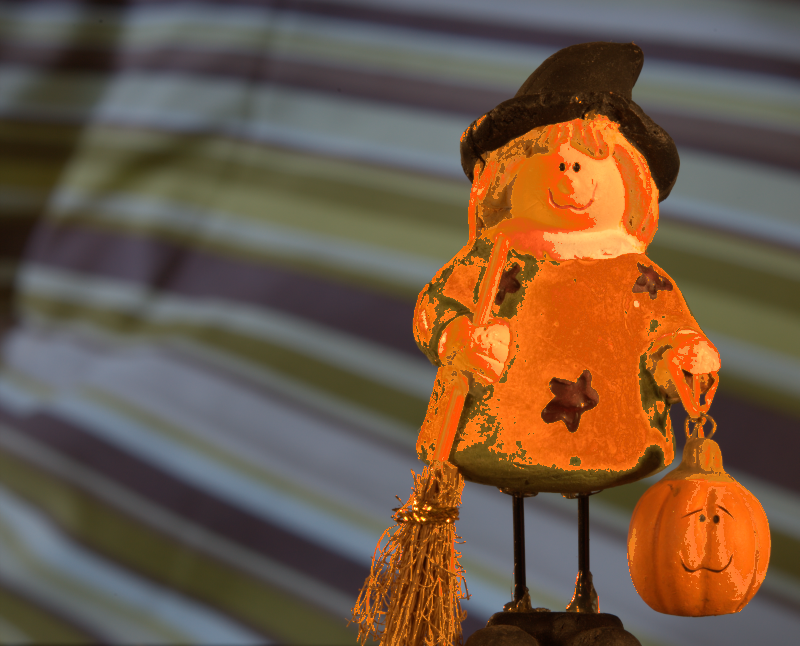
\includegraphics[scale=0.4]{img/matting-global_gegl_in_gimp.png}
\caption{Resultat der GEGL-Operation innerhalb von GIMP}
\label{fig:CE_gegl}
\end{figure}

%Bild Eingabe (Duck / matting-global / car-stack?)
%Vergleich Ausgabe bei Eingabe mit gleichen Parametern GIMP – GEGL Bilder
%Ergebnis vom Diff
\paragraph{Laufzeit}
Verwendet man zwei OpenMP-Threads, so wird der Code minimal schneller ausgeführt als mit einem Thread\footnote{Zur Ermittlung der Laufzeit wurde der Code jeweils 50 mal ausgeführt und die Laufzeit erfasst. Das Testsystem hierfür war Ubuntu 13.12 auf einem Q9550 mit 8 GB RAM. Auf die Verwendung des Institusrechners für Benchmarking wurde verzichtet.}, wie in \autoref{fig:CE_2} zu sehen ist. Dieser kaum merkliche Geschwindigkeitszuwachs rechtfertigt die gestiegene Code-Komplexität jedoch in keiner Weise.

Entgegen unseren Erwartungen wird dieses Filter mit zunehmender Anzahl an Threads langsamer statt schneller. Insbesondere bei der Ausführung mit vier Threads wird dieses Verhalten besonders deutlich.(siehe \autoref{algo:exchange_par}) Somit muss die Verwendbarkeit dieser Parallelisierungsstrategie für die praktische Nutzung entschieden verneint werden.
\begin{figure}[H]
\centering
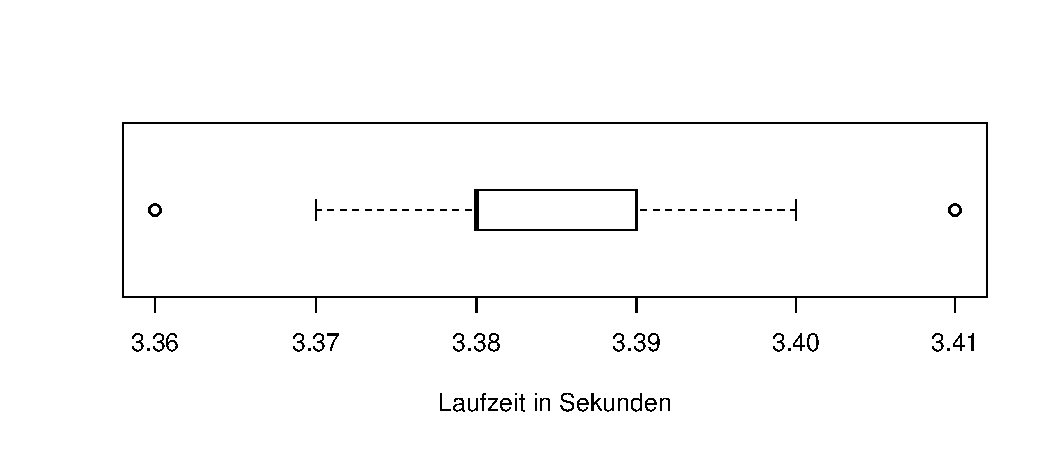
\includegraphics[scale=0.7]{graphs/seq.pdf}
\caption{Laufzeit von Color Exchange in der sequenziellen Implementierung}
\label{fig:CE_seq}
\end{figure}
\begin{figure}[H]
\centering
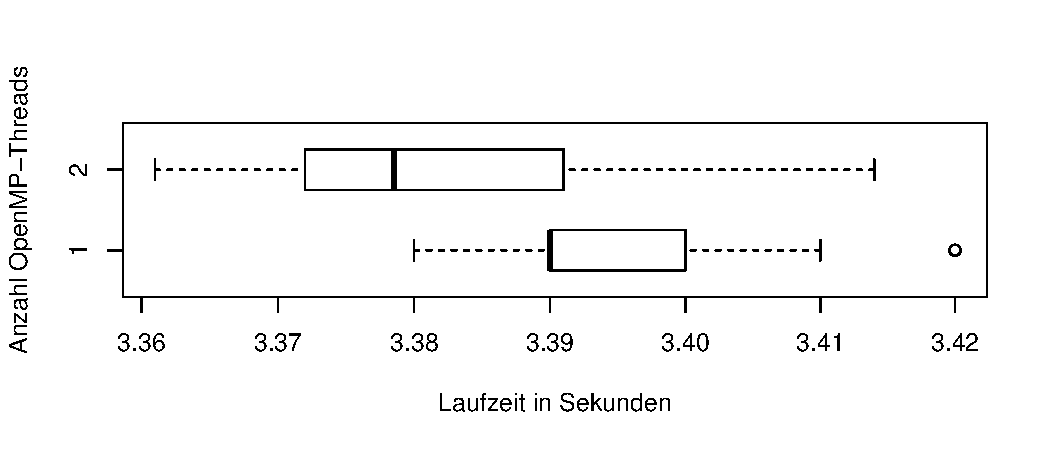
\includegraphics[scale=0.7]{graphs/diag_2threads.pdf}
\caption{Laufzeit von Color Exchange mit einem und zwei OpenMP-Threads}
\label{fig:CE_2}
\end{figure}

\begin{figure}[H]
\centering
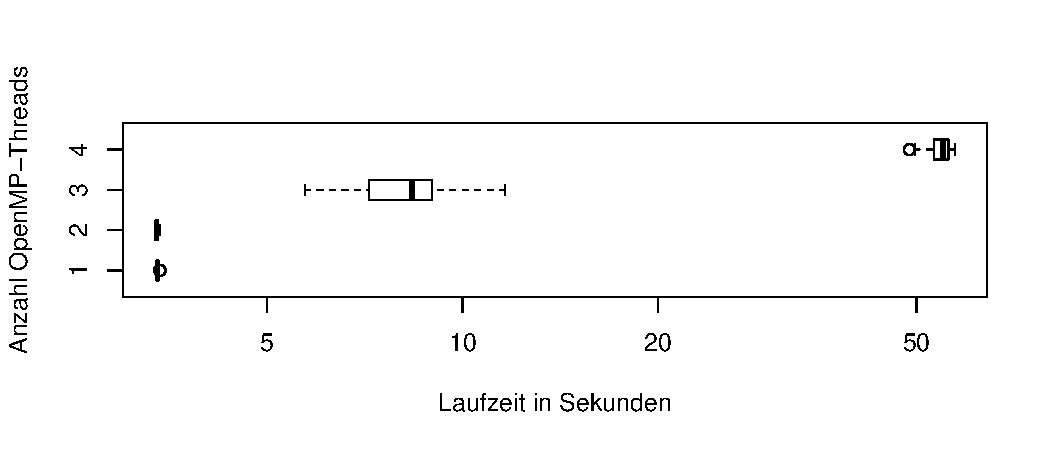
\includegraphics[scale=0.7]{graphs/diag.pdf}
\caption{Laufzeit von Color Exchange mit einem bis vier OpenMP-Threads}
\end{figure}
\begin{table}[H]
\centering
\begin{tabular}{lrrrrr}
\toprule
 & & \multicolumn{4}{c}{OpenMP-Threads} \\
\cmidrule(r){3-6}
 & seq & 1 & 2 & 3 & 4 \\
oberes Quartil 	& 3.39 		& 3.40 		& 3.3910 		& 8.973 		& 55.978 \\
Median 			& 3.38 		& 3.39 		& 3.3785 		& 8.360 		& 54.888 \\
unteres Quartil 	& 3.38 		& 3.39 		& 3.3720 		& 7.178 		& 53.18 \\
\bottomrule
\end{tabular}
\caption{Laufzeit von Color Exchange in verschiedenen Konfigurationen}
\label{tab:CE_runtime}
\end{table}
%X Durchläufe in Diagram abtragen?
%System beschreiben (Hardware, Software, Umgebungsvariablen) !!!
%Boxplots !!!
%Statistische Analyse ?!
%Aus Debug-Output Diagramm erstellen um Anteil des Filters an Gesamtlaufzeit zu verdeutlichen
%\subsection{Glass Tile}
%\paragraph{Korrektheit}
%Bild Eingabe (Duck / matting-global / car-stack?)
%Vergleich Ausgabe bei Eingabe mit gleichen Parametern GIMP – GEGL Bilder
%Ergebnis vom Diff
%\paragraph{Laufzeit}
%X Durchläufe in Diagram abtragen?
%System beschreiben (Hardware, Software, Umgebungsvariablen) !!!
%Boxplots !!!
%Statistische Analyse ?!
%Aus Debug-Output Diagramm erstellen um Anteil des Filters an Gesamtlaufzeit zu verdeutlichen
\subsection{Glass Tile}
\paragraph{Korrektheit}
Die Korrektheit der Implementierung des portierten Algorithmus wurde mithilfe der Gegl-Testumgebung geprüft mit dem Ergebnis, dass für verschieden gewählte Parameter stets eine Übereinstimmung mit dem GIMP-Referenzbild besteht.

\paragraph{Laufzeit}
Das Testsystem ist ein Intel Core-2-Duo 2,2 GHz Notebook mit zwei Kernen, 2GB RAM und Linux Ubuntu 13.04 als Betriebsystem. Als Testbild wurde ein 5000x3450 Pixel großes png-Bild mit 21 MB Dateigröße verwendet. Als Umgebungsvariablen für Gegl wurden die Default-Werte verwendet. Es wurden jeweils 50 Testläufe durchgeführt, sowohl für die sequentielle Version, als auch für ein bzw. zwei Threads in der parallelen Version. Die Ergebnisse werden in Abbildung~\ref{fig:gtile-runs} aufgezeigt. Man sieht, dass die parallele Version etwas schlechter abschneidet als die sequentielle. Die Parallelisierung dieses Filters lohnt sich demnach nicht.

\begin{figure}[h]
\begin{center}
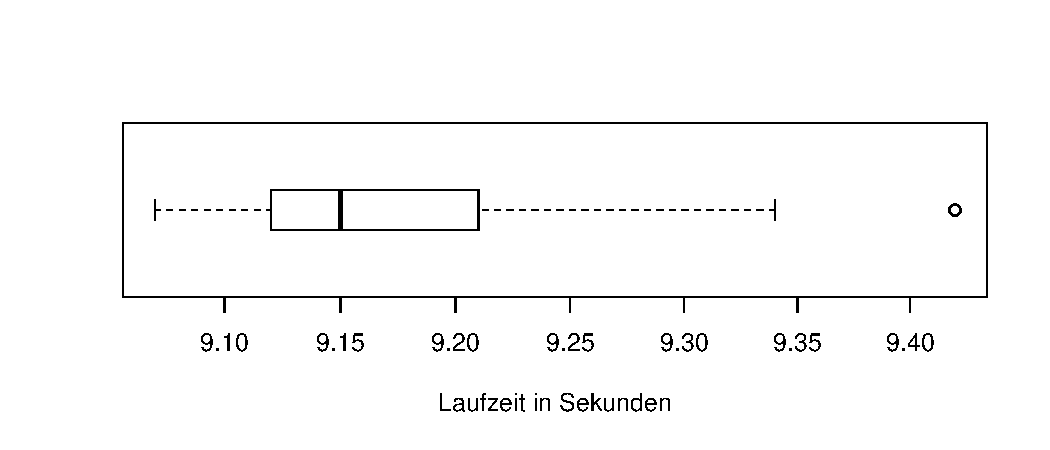
\includegraphics[width=1.0\textwidth]{graphs/glass-tile_seq.pdf}\newline
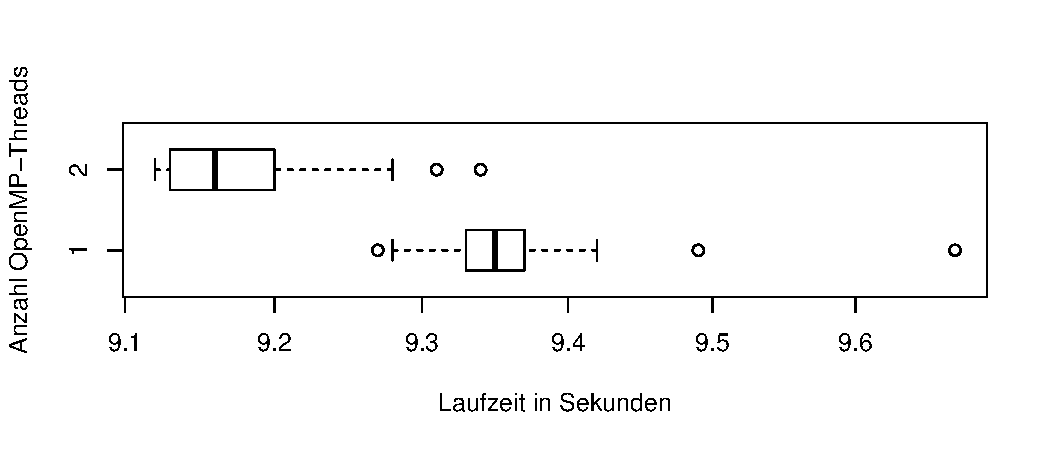
\includegraphics[width=1.0\textwidth]{graphs/glass-tile_2threads.pdf}
\end{center}
\caption{Laufzeit von Glass Tile (sequ. Variante oben, parallele Variante unten)}\label{fig:gtile-runs}
\end{figure}

Für die exemplarische detaillierte Ansicht der einzelnen Gegl-Aufrufe und die zugehörige Zeitmessung wurde jeweils ein Aufruf gemacht, bei dem \emph{GEGL-DEBUG-TIME} auf \emph{TRUE} gesetzt war. Wie in Abbildung~\ref{fig:gtile-dias} zu sehen ist, macht die eigentliche Operation nur einen Bruchteil der Gesamtzeit aus und die parallele Version benötigt länger als die sequentielle Version, was bereits weiter oben angedeutet wurde. Die sequentielle Variante gegl:tile-glass-seq wird in 0,73 sek ausgeführt, wohingegen die parallele Version mit 2 Threads gegl:tile-glass in 0,85 sek läuft.

\begin{figure}[h]
\begin{center}
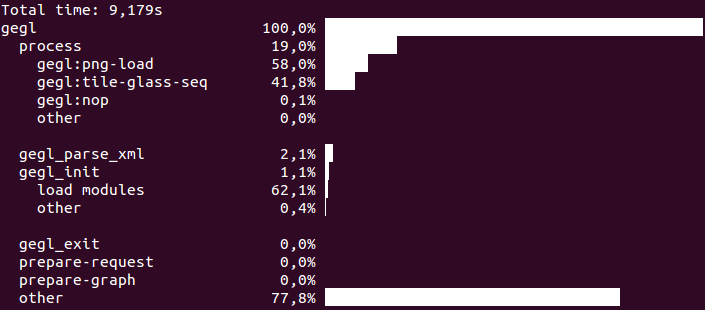
\includegraphics[width=1.0\textwidth]{gtile_seq_dia.png}
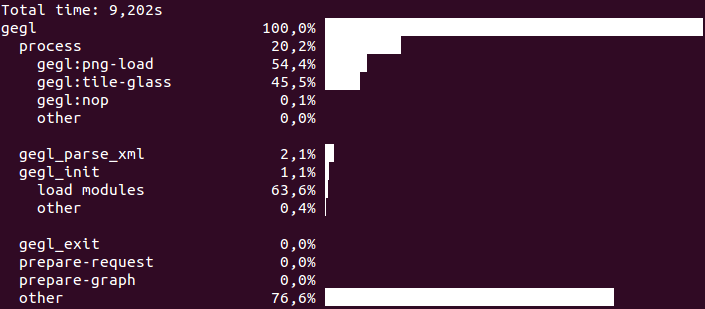
\includegraphics[width=1.0\textwidth]{gtile_par_dia.png}
\end{center}
\caption{Detailansicht der Gegl-Aufrufe (sequ. Variante oben, parallele Variante mit 2 Threads unten)}\label{fig:gtile-dias}
\end{figure}



%\subsection{Neon}
%\paragraph{Korrektheit}
%Bild Eingabe (Duck / matting-global / car-stack?)
%Vergleich Ausgabe bei Eingabe mit gleichen Parametern GIMP – GEGL Bilder
%Ergebnis vom Diff
%\paragraph{Laufzeit}
%X Durchläufe in Diagram abtragen?
%System beschreiben (Hardware, Software, Umgebungsvariablen) !!!
%Boxplots !!!
%Statistische Analyse ?!
%Aus Debug-Output Diagramm erstellen um Anteil des Filters an Gesamtlaufzeit zu verdeutlichen
\newpage
%% edge-neon_teil2.tex
\subsection{Neon}
\paragraph{Korrektheit}
\label{paragraph:neon_korrektheit}
%Bild Eingabe (Duck / matting-global / car-stack?)
%Vergleich Ausgabe bei Eingabe mit gleichen Parametern GIMP – GEGL Bilder
%Ergebnis vom Diff
Trotz sehr aufwändiger Suche und Behandlung, auch mehrfaches Neuanfangs konnten wir einen Fehler bei der Kachelzerlegung nicht fixen.  
Unerwarteter Weise werden horizontale Kachelränder etwas verzerrt, wobei in den allermeisten Bildern die angesprochene Verzerrung so unauffällig ist, dass man nach dieser gezielt suchen muss.
Anscheinend behandelt GEGL diesen Punkt nicht gleichermaßen wie GIMP.
Da wir aber auch dieses Filter gern commiten würden, werden wir uns mit GEGL-Leuten in Verbindung setzen und um Hinweise bitten.

Wird das Bild nur in senkrechte oder keine Kacheln zerlegt, so stimmen die Ausgaben von GEGL und GIMP überein.
\paragraph{Laufzeit}
%X Durchläufe in Diagram abtragen?
%System beschreiben (Hardware, Software, Umgebungsvariablen) !!!
%Boxplots !!!
%Statistische Analyse ?!
%Aus Debug-Output Diagramm erstellen um Anteil des Filters an Gesamtlaufzeit zu verdeutlichen
Tabelle \ref{tab:NEON_runtime} enthält wichtigste Daten über die Laufzeit dieses Filters in verschiedenen Konfigurationen. 

Manche Messungen sind mit schedule(dynamic) durchgeführt, solche sind mit dem ``d''-Zeichen neben der Threadszahl markiert. Wie man der Tabelle entnehmen kann, liegt der entstehende Vorteil durch schedule(dynamic) mit 4 Threads unter 1\%. Bei einer geringeren Threadszahl zeigt sich dynamische Aufteilung bediengt durch Overhead sogar störend (nicht in der Tabelle aufgelistet).

Der ursprünglich verfolgte Ansatz ``Sections'' konnte  unsere Erwartungen leider nicht erfüllen, und schließt die Liste in allen Tests ab. Eine wichtige Anmerkung an dieser Stelle ist, dass für innere Parallelität hier SET\_NESTED=TRUE essentiell ist.

Der konservative Ansatz zeigte sich im Gegenteil zu Section sehr gut. Hier lässt sich eine Abhängigkeit zwischen Threadszahl und der ausgewählten Methode beobachten. Während Ansatz ohne Datenabhängigket (mit zusätzlichen Buffern) sich am besten mit wenigen Threads zeigt, konnte der Ansatz mit Datenabhängigkeit(ohne zusätzliche Buffer) unsere Tests mit 4 Threads am besten abschneiden(unabhängig von Scheduler und Bildgröße).


Alle Angaben in Sekunden. Messungen an Intel i5-3570 CPU mit 4 physikalischen Kernen (4 Threads) @ 3.40GHz und 6144 KB L2-Cache, ausgerüstet mit 8 Gb RAM (1600 Mhz) unter Ubuntu 13.10. Gemessen wurde aber nur allgemeine Zeit: mit GEGL aufrufen, mit Bild einlesen, mit Bild abspeichern - nur diese Angaben sind für den Endnutzer interessant.

Info über verwendete Bilder:

raupe.png 6023x3645 Pixel, 7.5 MB

wolf.png 2620x1503 Pixel, 322.8 kB

lenna.png 512x512 Pixel
\begin{table}[h] 473.8 kB
\centering
\begin{tabular}{c p{2cm}p{2cm}p{2cm}}
\toprule
\textbf{\#Thread} & \textbf{Lenna} & \textbf{Wolf} & \textbf{Raupe} \\

\cmidrule(r){1-4}

\multicolumn{4}{c}{Conservative (ohne DA, static)} 	\\
4d 	& 0.252		&1.124		&6.822			\\
4 	& 0.252		&4.123		&6.960 		 	\\
2	& 0.270		&1.454		&8.603			\\
1	& 0.314		&2.157		&12.438 			\\

\cmidrule(r){1-4}

\multicolumn{4}{c}{Sections (ohne DA, static)} 		\\
2*2 	& 0.254		&1.222		&7.412 		 	\\
2*1	& 0.280		&1.571		&9.366 		 	\\

\cmidrule(r){1-4}

\multicolumn{4}{c}{Conservative (mit DA, static)}	\\
4d	& 0.246		& 1.126		& 6.761			\\
4 	& 0.248		&1.139		& 6.792		 	\\
2	& 0.268		&1.471		& 8.685 		 	\\
1	& 0.318		&2.203		&12.772			\\

\bottomrule
\end{tabular}
\flushleft{
\footnotesize{\textsuperscript{*} ein ``'d'-Zeichen neben der Threadszahl weist darauf hin, dass diese Laufzeit mit schedule(dynamic) gemessen wurde, ansonsten mit schedule(static)
}}
\caption{Laufzeit von Neon in verschiedenen Konfigurationen}
\label{tab:NEON_runtime}
\end{table}

Zusammenfassend kann man volgendes sagen:
\begin{itemize}
\item Sections sind in diesem Filter eher ungeeignet (allgemeine Tests ob sections in OpenMP effizient abgearbeitet werden wären erwünscht).
\item Bei geringen Threadszahlen ist der konservative Ansatz mit Datenabhängigkeit wegen der besseren Cache-Ausnutzung (vgl. zu Kapitel \ref{paragraph:neon_filter}:Parallelisierung) die beste Wahl.
\item Mit steigender Threadszahl wird der konservative Ansatz ohne Datenabhängigkeit zum Spitzenreiter.
\item Erzielter SpeedUp: Beste allgemeine 1-Thread-Zeit/Beste allgemeine 4-Thread-Zeit
lenna: 1.2764, wolf: 1.9190, raupe: 1.8312
\end{itemize}






\subsection{Selective Gaussian Blur}
\paragraph{Korrektheit}
%Bild Eingabe (Duck / matting-global / car-stack?)
%Vergleich Ausgabe bei Eingabe mit gleichen Parametern GIMP – GEGL Bilder
%Ergebnis vom Diff
\paragraph{Laufzeit}
%X Durchläufe in Diagram abtragen?
%System beschreiben (Hardware, Software, Umgebungsvariablen) !!!
%Boxplots !!!
%Statistische Analyse ?!
%Aus Debug-Output Diagramm erstellen um Anteil des Filters an Gesamtlaufzeit zu verdeutlichen
%Warum wird es mit OpenMP langsamer?
\section{Abschließende Betrachtung}
Einen unerwartet großen Anteil an der aufgewandten Zeit hat die Portierung in Anspruch genommen. Insbesondere das Verständnis für die Funktionsweise von GEGL und den Unterschieden der Farbräume hat sich erst nach tiefgründiger Beschäftigung eingestellt. Waren dann GEGL und der zu portierende Algorithmus erst einmal verstanden lief die Portierung relativ flüssig ab. Das Tiling durch GEGL hat jedoch hin und wieder für längere Denkpausen gesorgt.

Positiv ist anzumerken, dass die Quellcode-Dateien infolge der Portierung nach GEGL deutlich übersichtlicher geworden sind, da der ganze Code für in allen Filtern wiederkehrende Aufgaben wie z.B. GUI-Erstellung und Aktualisierung, wegfällt.

Die Parallelisierung mittels OpenMP ist sicherlich nicht die optimale Lösung für GEGL-Filter, da das Tiling eigentlich als Parallelisierungsmechanismus vorgesehen ist. Somit ist ein Teil der Parallelisierung eher als akademische Übung zu betrachten. Nichtsdestotrotz dürfte für jedes Mitglied der Gruppe ein Informations- und Erfahrzungsgewinn zu verzeichnen sein. Insbesondere die Integration in den Entwicklungsprozess eines Open-Source-Projektes fand viel Zustimmung und war ein motivierender Faktor.

\section{Ausblick}
Viele Filter warten noch darauf von GIMP nach GEGL portiert zu werden. Die gesammelten Erfahrungen aus der bereits durchgeführten Portierung werden weitere sicherlich begünstigen.

Aber auch bei den bereits portierten Filtern gibt es teilweise noch Raum für Verbesserungen. So könnten auch die restlichen Filter nach OpenCL portiert werden, es gibt in den GIMP-Filtern diverse kleine Bugs beziehungsweise Verhalten, dass man als Nutzer nicht erwarten würde. In Absprache mit der GIMP- und GEGL-Community werden wir auch nach Abschluss der vorliegenden Arbeit sicherlich noch die ein oder andere Zeile Code in GEGL einfließen lassen.

Unsere Portierungen werden wir von den OpenMP-Konstrukten bereinigt als Patches für das GEGL-Projekt einreichen. Die Vorgehensweise hierfür wurden bereits mit GEGL-Entwicklern abgesprochen, sodass von einer baldigen Erledigung auszugehen ist.
%Umstellung auf Floats
%Behebung des Bugs
%Implementierung in OpenCL
\section{Grußworte}
Wir bedanken uns an dieser Stelle bei der GIMP- und GEGL-Community, die nicht nur diese äußerst nützlichen Software-Produkte entwickeln und der Menschheit frei und quelloffen zur Verfügung stellen sondern auch zu jeder Tages- und Nacht-Zeit sehr schnell mit hilfreichen Antworten auf Fragen zur Seite standen. Auch bei Thomas und Luis, den Betreuern dieser Arbeit, wollen wir uns an dieser Stelle für die motivierte und fundierte Betreuung bedanken.
\end{document}
